\section{Fluxions} \label{chapter5:flx}

The previous section presented a compiler to identify and extract the underlying pipeline in a Javascript application.
However, the stages doesn't enforce the isolation required for parallel execution.
Moreover, the Dues that constitues the stages of this pipeline 

only parts of the pipeline are identified, 
This section present the second contribution of this thesis.
The equivalence between a memory shared among all the operations and independent memory for each operation in a pipeline.
It tackles the problems arising from the translation of the global memory synchronization into message passing.

This equivalence is implemented as a compiler, improving upon the previous one.
The compiler transforms a Javascript application into a network of independent parts communicating by message streams and executed in parallel.
We named these parts \textit{fluxions}, by contraction between a flux and a function.
% Fluxions are executed in an execution model that assure parallelism and communications.

% We present an early version of this tool as a proof of concept for this compilation approach.
% Section \ref{chapter5:flx:model} describes the execution model that executes fluxions in parallel, and assure their communications.

The identification of the rupture points between fluxions is addressed in section \ref{chapter5:flx:compiler}.
The isolation between the fluxions, after identification, is addressed in section \ref{chapter5:flx:isolation}.
% The compiler, and the equivalence are described in section \ref{chapter5:flx:compiler}.
Section \ref{chapter5:flx:evaluation} presents a real-case test of compilation, and expose the limits of this compiler.

% # Explanation of the concept

% ## Turn-based programming.

% (see presentation on Dues)
% -> single-thread, no wait, no block and so on
% Shared heap -> no mutex, no synchronization, so it is good scalability


% Turn-based programming is an event-loop.
% It is the execution of queued events one after the other.
% An event is the association of a callback and a message.
% The callback is a small Javascript Program, designed to process the message.
% During its turn, the callback executes, and can queue events : that is register callback to be executed during a next turn.
% TODO what I mean exactly by queue events ? -> the distinction between the asynchronous operation, and the resulting event.

% ## Pipeline

% So a callback sends messages to other callbacks.
% -> It is exactly like a pipeline.
% However, all the callbacks share the same heap.
% So it is not possible to distribute the different callbacks without synchronization of this heap, or splitting the heap for each callback.
% TODO state VERY clearly this problem, it is at the core of my thesis.

% So, how to split the heap so that each callback has its own exclusive heap ?

\comment{From here, the reader should be confortable with the event-loop, and the analogy we drawn between the event-loop and a pipeline.
The problematic is now clear : how to split the heap so that each asynchronous callback has its own exclusive heap ?}

\section{Callback identification}

\subsection{\comment{TODO}}

\section{Callback isolation}

We explain in this section the compilation process we developped to isolate the memory access for each callbacks.
The result of this process should be two-fold. First each callback should have an exclusive access on a region of the memory. So that two different callback can be executed in parallel. And it should be clear for each callback, what are the variable needed from upstream callbacks, and what are the variable to send downstream.

\subsection{Propagation of variables}


\subsubsection{Scope identification}

In section \ref{??? Javascript scope / closure}, we explained that Javascript is roughly lexically scoped.
A consequence is that the declaration of contexts can be inferred statically.
For example, in a lexically scoped, strongly typed, compiled language, the compiler know the content of each scope during compile time, and can prepare the memory stack to store the variables in each scope.

In most languages, the memory is in two parts : the stack, and the heap.
The stack is statically scoped, and its layout is known at compile time.
The heap, on the other hand is dynamically allocated. Its layout is built at run time.

But Javascript is a dynamic language, perhaps the most dynamic of all languages.
It doesn't have this distinction between stack and heap. Every variable is dynamically allocated on the heap.
That induce two consequences.
The first is that Javascript provides two statements to dynamically modify the lexial scope : \texttt{eval} and \texttt{with}.
The second is that to know the layout of the heap, we need to use static analysis tools.
In the next two sections, we adress these two consequences.

\subsubsection{Break the lexical scope} \label{???:breakscope}

Without these statements, \texttt{eval} and \texttt{with}, Javascript is lexically scoped. It is possible to infer the scope of each variable at compile time.


The \texttt{with} statement continue the execution using an expression as the lexical scope.
As the provided expression is dynamically evaluated, it is possible to dynamically modify the lexical scope.
The code snippet below show an example of such a situation.

\begin{code}
var aliveCat = {isAlive: true};
var deadCat = {isDead: true}

with (Math.random() > 0.5 ? aliveCat : deadCat) {
  isAlive;
  // Half the time -> ReferenceError: isAlive is not defined
  // Half the time -> true;
}
\end{code}

The variable \texttt{isAlive} is defined only in the object \texttt{aliveCat}.
The presence of the variable \texttt{isAlive} in the lexical environment within the \texttt{with} statement cannot be determined statically, as the lexical environment is dynamically linked to either \texttt{aliveCat} or \texttt{deadCat}.

Note that the MDN reference page on \texttt{with}\ftnt{https://developer.mozilla.org/en-US/docs/Web/JavaScript/Reference/Statements/with} says that \textit{Using \texttt{with} is not recommended, and is forbidden in ECMAScript 5 strict mode.}

The \texttt{}

% TODO and specify that Javascript is roughly lexically scoped : it is not completely lexically scoped, and five examples to backup that.

Not to be mistaken with the \texttt{this} operator.
It is possible to dynamically change the content of an object,  
% TODO continue this paragraph about how the this operator change the properties of an object. 
% Does it change the lexical scope, if that object is actually used as a context elsewhere ? -> No, I don't think so.
% But ask on SO, just to be sure.

\begin{code}
function stuff() {
  this.x = 42;
}

stuff.call({})

\end{code}

% Javascript is lexically scoped, therefore we can identify the the scope of variable statically.
% (At the exception of eval and with : with is forbidden from strict mode, so that is not a bigdeal, howether, eval is sometimes used in smart ways, but most of the time it is monomorphic (I don't exactly know what that means, I heard from Floreat, it must be something related to PL community)).

% The compiler identifies the variables shared by multiple callbacks from their scope.
% TODO explain this in depth.
% Function scope, closures, and so on ...



However, even if Javascript is lexically scoped, the memory is still dynamicall allocated and manipualeted, so that it is not possible to actually infer the memory layout at compiler time only with lexical scope analysis, and without deeper static analysis.

\subsubsection{Scope Leaking}

% Javascript uses a pass-by-sharing paradigm.
% That means that sometimes the argument of a call are passed by value, sometimes by reference (atomic data type (number, string, bool) -> by value, complex data type (objects) -> by reference).
% That means that the modification of a local variable can affect variable in seemingly unrelated scopes.
% It seems that the points-to analysis is what is used to find stuffs like that (side-effects ?).

% TODO what we are talking about here are aliases.

% TODO I am stating here that in low-level language, the memory access is so fine, that it is difficult to exactly pin down the memory layout in term of object, it is rather seen as a big array of memory adresses.
% While in higher-level language, like Javascript, the memory access is at the property level (it is not possible to access memory down to the adress), so it could be easier (maybe, just not harder) to infer the dynamic memory layout from source.
To infer the layout of the heap at compile time, static analysis tools are used, like the points-to analysis, developped by Andersen in its PhD thesis \cite{Andersen1994}.
For such analysis, the memory is splitted at the access scale.
In low-level languages, like C/C++, the memory is mainly managed by the developer. Allowing access to the memory at a small grained scale : up to the address.
It impose the analysis to split the memory to the adress scale in some cases.
% TODO Backup that, HEAVILY
In higher-level languages, like Javascript, the developer cannot access the memory to the adress scale.
The memory is accessed at a coarser scale : the property scale.
(At the exception of some arrays and buffers, that mimic, and are mapped to actual memory adresses for performance reasons.)
% TODO find exactly the references for these buffers : I think of ArrayBuffer, and sharedArray ... but I am not sure. Need more inspection.

\subsubsection{Propagation of execution and variables}

For the execution of each callback / stage, the corresponding part of the state is local, and the rest is remote, and inaccessible.
We are going to explain why it must remain inaccessible.

While a callback is executing a request, the previous callback (the up stream callback) is executing the next request.
The next request will arrive at the current callback some time in the future.
The modification done in the state of the upstream callback will propagate only later in the current callback.
The state of the upstream callback is in a different time frame than the state of the current callback.

To really understand that, we need to compare this execution with the execution on a unique event-loop.
If the current callback executes, then the upstream callback might have, or might not have started to execute the next request.
But as soon as the current callback executes, the modifications done on the states, are immediatly propagated, so that the upstream callback can take them into account for the next request.

However, if the two callbacks are distant, then the modification of the current callback will not immediatly propagate to the upstream callback.
During the propagation, the upstream callback might execute requests than would not be aware of the state modification from the current callback (from downstream).
That is why we say the upstream callback and the current callback are in two different time frame.
Propagating the state modification upstream is like going backward in time, it is impossible.
That is why the execution, and the state modification propagation must always flow downstream.

As a note, I must add that if an upstream and a downstream callbacks are on the same event-loop, then this doesn't apply. it is like a loop in the time : the modification immediatly propagate from downstream to upstream.






% The execution progress downstream, following the message stream.
% TODO state very clearly this proposition, it is the second core of my thesis (and I love the idea, it relates directly to reality, graivity, and the fabric of the universe <3).

% Because the propagation of the modification is not instantaneous, going back upstream is like going backward in time : it is impossible.
% Therefore, a variable cannot be read upstream a write.
% And it cannot be write downstream either.

% In other words, only one callback can write on a variable -> seems obvious from previous sections.


% In promises, because the heap is not shared, things are less restrictive.
% Multiple stages can read and write the same variable, because the propagation of modification is instantaneous, due to the shared heap.





% TODO write about what it implies to detect continuation in variable, or other expressions.

% Why can we only detect continuations declared in situ.
% If a continuation is passed as a variable, we don't know for sure what is the function associated with, and the closure of that function.

\subsection{Fluxions Isolation} \label{chapter5:flx:isolation}

As a rupture point occurs between an asynchronous caller and a callback defined \textit{in situ}, it eventually breaks the chain of scopes.
% A rupture point eventually breaks the chain of scopes between the upstream and downstream fluxion.
If the caller and the callback are separated, it breaks the closure of the callback.
The callback in the downstream fluxion cannot access the scope of its parent as expected. % in the upstream fluxion.
% The closure in the downstream fluxion cannot access the scope in the upstream fluxion as expected.
The pipeliner step replaces the need for this closure, allowing application parts to be isolated, and to rely only on independent memory stores and message passing.
It determines the distribution using the scope representation, which represents the variables' dependencies between application parts.
Depending on this representation, the compiler can replace the broken closures in three different ways.
We present these three alternatives in figure \ref{fig:states}.

\begin{figure}[h!]

\bigfig{
  \centering
  \parbox{\textwidth}{
    \parbox{0.40\textwidth}{
      \hfill
      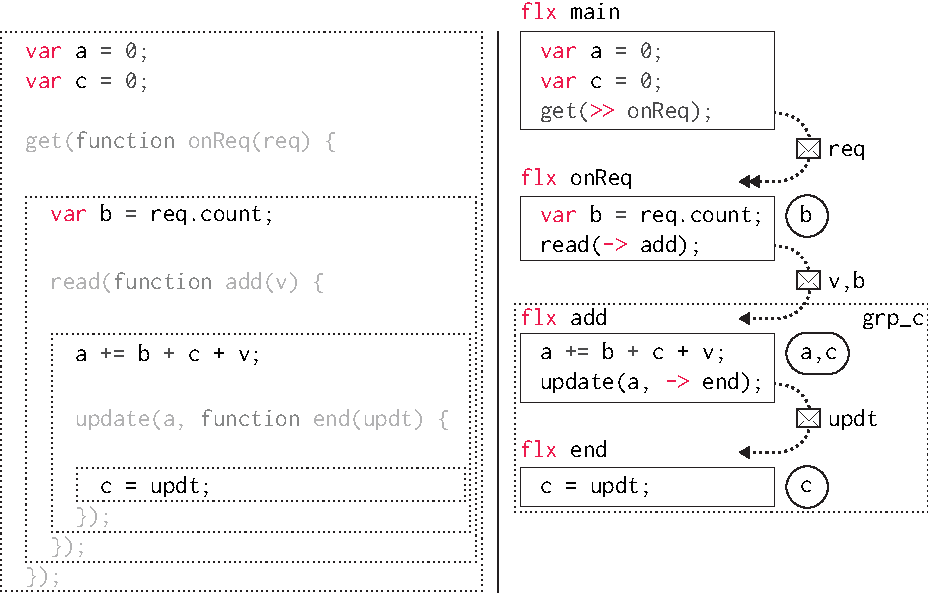
\includegraphics[page=1, height=0.4\textwidth]{../resources/states.pdf}
    }
    \hspace{10pt}
    $\to$
    \hspace{10pt}
    \parbox{0.40\textwidth}{
      \includegraphics[page=2, height=0.4\textwidth]{../resources/states.pdf}
      \hfill
    }
    \caption{Variable management from Javascript to the high-level fluxional language}
    \label{fig:states} 
  }
}

\end{figure}

\paragraph{Scope}
If a variable is modified inside only one application part in the current \textit{post} chain, then the pipeliner adds it to the context of its fluxion.

In figure \ref{fig:states}, the variable \texttt{a} is updated in the function \texttt{add}.
The pipeliner step stores this variable in the context of the fluxion \texttt{add}.

\paragraph{Stream}
If a modified variable is read by some downstream application parts, then the pipeliner makes the upstream fluxion add this variable to the message stream to be sent to the downstream fluxions.
It is impossible to send variables to upstream flux\-ions, without causing inconsistencies.
If the fluxion retro propagates the variable for an upstream fluxion to read, the upstream fluxion might use the old version while the new version is on its way.

In figure \ref{fig:states}, the variable \texttt{b} is set in the function \texttt{onReq}, and read in the function \texttt{add}.
The pipeliner step makes the fluxion \texttt{onReq} send the updated variable \texttt{b}, in addition to the variable \texttt{v}, in the message sent to the fluxion \texttt{add}.

Exceptionally, if a variable is defined inside a \textit{post} chain, like \texttt{b}, then this variable can be streamed inside this \textit{post} chain without restriction on the order of modification and read.
Indeed, in the current \textit{post} chain, the execution of the upstream fluxion is assured to end before the execution of the downstream fluxion, because of their causality.
Therefore, no reading of the variable by the upstream fluxion happens after the modification by the downstream fluxion.

\paragraph{Share}
If a variable is needed for modification by several application parts, or is read by an upstream application part, then it needs to be synchronized between the fluxions.
% To respect the semantics of the source application, we cannot tolerate inconsistencies.
The pipeliner groups all the fluxions sharing this variable with the same tag.
And it adds this variable to the contexts of each fluxions.

In figure \ref{fig:states}, the variable \texttt{c} is set in the function \texttt{end}, and read in the function \texttt{add}.
As the fluxion \texttt{add} is upstream of \texttt{end}, the pipeliner step groups the fluxion \texttt{add} and \texttt{end} with the tag \texttt{grp\_c} to allow the two fluxions to share this variable.
\subsection{Real test case} \label{chapter5:flx:evaluation}

The compiler is tested on a real application, gifsockets-server\ftnt{https://github.com/twolfson/gifsockets-server}.
This test proves the possibility for an application to be compiled into a network of independent parts.
It shows the current limitations of this isolation and the modifications needed on the application to circumvent them.

\begin{code}[js, caption={Simplified version of gifsockets-server},label={lst:gifsocket}]
var express = require('express'),
    app = express(),
    routes = require('gifsockets-middleware'), //@\label{lst:gifsocket:gif-mw}@
    getRawBody = require('raw-body');

function bodyParser(limit) { //@\label{lst:gifsocket:bodyParser}@
  return function saveBody(req, res, next) { //@\label{lst:gifsocket:saveBody}@
    getRawBody(req, { //@\label{lst:gifsocket:getRawBody}@
      expected: req.headers['content-length'],
      limit: limit
    }, function (err, buffer) { //@\label{lst:gifsocket:callback}@
      req.body = buffer;
      next(); //@\label{lst:gifsocket:next}@
    });
  };
}

app.post('/image/text', bodyParser(1 * 1024 * 1024), routes.writeTextToImages); //@\label{lst:gifsocket:app.post}@
app.listen(8000);
\end{code}

This application, simplified in listing \ref{lst:gifsocket}, is a real-time chat using gif-based communication channels.
It was selected from the evaluation set of the Due compiler because it is simple enough to illustrate this evaluation.
% \cite{Brodu2015}
%  from the \texttt{npm} registry because it depends on \texttt{express}, it is tested, working, and simple enough to illustrate this evaluation.
The server transforms the received text into a gif frame, and pushes it back to a never-ending gif to be displayed on the client.

On line \ref{lst:gifsocket:app.post}, the application registers two functions to process the requests received on the url \texttt{/image/text}.
The closure \texttt{saveBody}, line \ref{lst:gifsocket:saveBody}, returned by \texttt{bodyParser}, line \ref{lst:gifsocket:bodyParser}, and the method \texttt{routes.write\-Text\-To\-Images} from the external module \texttt{gifsockets-\-middleware}, line \ref{lst:gifsocket:gif-mw}.
The closure \texttt{saveBody} calls the asynchronous function \texttt{getRawBody} to get the request body.
Its callback handles the errors, and calls \texttt{next} to continue processing the request with the next function, \texttt{routes.write\-Text\-To\-Images}.

\subsubsection{Compilation} \label{chapter5:flx:evaluation:compilation}

% We compile this application with the compiler
The compilation result is in listing \ref{lst:flx-gifsocket}.
The function call \texttt{app.post}, line \ref{lst:gifsocket:app.post}, is a rupture point.
However, its callbacks, \texttt{bodyParser} and \texttt{routes.write\-Text\-To\-Images} are not declared \textit{in situ}.
They are evaluated as functions only at runtime.
As precised previously, the compiler discards these callbacks to avoid altering the semantic. % by moving or modifying their definition.
% For this reason, the compiler ignores this rupture point, to avoid interfering with the evaluation.

\begin{code}[flx, caption={Compilation result of gifsockets-server},label={lst:flx-gifsocket}]
flx main & express {req}
>> anonymous_1000 [req, next]
  var express = require('express'),
      app = express(),
      routes = require('gifsockets-middleware'), //@\label{lst:flx-gifsocket:gif-mw}@
      getRawBody = require('raw-body');

  function bodyParser(limit) { //@\label{lst:flx-gifsocket:bodyParser}@
    return function saveBody(req, res, next) { //@\label{lst:flx-gifsocket:saveBody}@
      getRawBody(req, { //@\label{lst:flx-gifsocket:getRawBody}@
        expected: req.headers['content-length'], //@\label{lst:flx-gifsocket:req.headers}@
        limit: limit
      }, >> anonymous_1000 [req, next]);
    };
  }

  app.post('/image/text', bodyParser(1 * 1024 * 1024), routes.writeTextToImages); //@\label{lst:flx-gifsocket:app.post}@
  app.listen(8000);

flx anonymous_1000
-> null
  function (err, buffer) { //@\label{lst:flx-gifsocket:callback}@
    req.body = buffer; //@\label{lst:flx-gifsocket:buffer}@
    next(); //@\label{lst:flx-gifsocket:next}@
  }
\end{code}

The compiler detects a rupture point : the function \texttt{get\-Raw\-Body} and its anonymous callback, line \ref{lst:gifsocket:callback}.
It encapsulates this callback in a fluxion named \texttt{anony\-mous\_\-1000}.
The callback is replaced with a stream placeholder to send the message stream to this downstream fluxion.
The variables \texttt{req} and \texttt{next} are appended to this message stream, to propagate their value from the \texttt{main} fluxion to the \texttt{anony\-mous\_\-1000} fluxion.

When \texttt{anony\-mous\_\-1000} is not isolated from the \texttt{main} fluxion, as if they belong to the same group, the compilation result works as expected.
The variables used in the fluxion, \texttt{req} and \texttt{next}, are still shared between the two fluxions.
In this situation fluxions are quite similar to Dues regarding memory shareing.
Our goal is to isolate the two fluxions, to be able to safely parallelize their executions.

\subsubsection{Isolation} \label{chapter5:flx:evaluation:isolation}

In listing \ref{lst:flx-gifsocket}, the fluxion \texttt{anony\-mous\_\-1000} modifies the object \texttt{req}, line \ref{lst:flx-gifsocket:buffer}, to store the text of the received request, and it calls \texttt{next} to continue the execution, line \ref{lst:flx-gifsocket:next}.
\texttt{req} is an alias to a memory location used in multiple palces in code.
Therefore, these operations produce side-effects that should propagate in the whole application, but the isolation prevents this propagation.
Isolating the fluxion \texttt{anony\-mous\_\-1000} produces runtime exceptions.
The next paragraph details how this situation is handled to allow the application to be parallelized.

\paragraph{Variable \texttt{req}}

The variable \texttt{req} is read in fluxion \texttt{main}, lines \ref{lst:flx-gifsocket:getRawBody} and \ref{lst:flx-gifsocket:req.headers}.
Then its property \texttt{body} is associated to \texttt{buffer} in fluxion \texttt{anony\-mous\_\-1000}, line \ref{lst:flx-gifsocket:buffer}.
The compiler is unable to identify the aliases of this variable. % further usages.
However, the side effect resulting from this association impacts a variable in the scope of the next callback, \texttt{routes.write\-Text\-To\-Images}.
In this test case, the application is modified manually to explicitly propagate this side-effect to the next callback through the function \texttt{next}.
The modifications of this function are explained further in the next paragraph.

\paragraph{Closure \texttt{next}}

The function \texttt{next} is a closure provided by the \texttt{express} \texttt{Router} to continue the execution with the next function to handle the client request.
Because it indirectly relies on the variable \texttt{req}, it is impossible to isolate its execution with the \texttt{anony\-mous\_\-1000} fluxion.
Instead, we modify \texttt{express}, so as to be compatible with the fluxional execution model.
We explain the modifications below.

\begin{code}[flx, caption={Simplified modification on the compiled result},label={lst:mflx-gifsocket}]
flx anonymous_1000
-> express_dispatcher
  function (err, buffer) { //@\label{lst:mflx-gifsocket:callback}@
    req.body = buffer; //@\label{lst:mflx-gifsocket:buffer}@
    next_placeholder(req, -> express_dispatcher); //@\label{lst:mflx-gifsocket:next-placeholder}@
  }

flx express_dispatcher & express {req} //@\label{lst:mflx-gifsocket:express-dispatcher}@
-> null
  function (modified_req) {
    merge(req, modified_req);
    next(); //@\label{lst:mflx-gifsocket:next}@
  }
\end{code}

In listing \ref{lst:gifsocket}, the function \texttt{next} is a continuation allowing the anonymous callback, line \ref{lst:gifsocket:callback}, to call the next function to handle the request.
To isolate the anonymous callback into \texttt{anonymous\_\-1000}, \texttt{next} is replaced by a rupture point.
This replacement is illustrated in listing \ref{lst:mflx-gifsocket}.
The \texttt{express} \texttt{Router} registers a fluxion named \texttt{express\_\-dispatcher}, line \ref{lst:mflx-gifsocket:express-dispatcher}, to continue the execution after the fluxion \texttt{anony\-mous\_\-1000}.
This fluxion is in the same group \texttt{express} as the \texttt{main} fluxion, hence it has access to the original variable \texttt{req}, and to the original function \texttt{next}.
The call to the original \texttt{next} function is replaced by a placeholder to push the stream to the fluxion \texttt{express\_\-dispatcher}, line \ref{lst:mflx-gifsocket:next-placeholder}.
The fluxion \texttt{express\_\-dispatcher} receives the stream from the upstream fluxion \texttt{anony\-mous\_\-1000}, merges back the modification in the variable \texttt{req} to propagate the side effects, and finally calls the original function \texttt{next} to continue the execution, line \ref{lst:mflx-gifsocket:next}.

After the modifications detailed above, the server works as expected.
The isolated fluxion correctly receives, and returns its serialized messages.
The client successfully receives a gif frame containing the text.



\subsection{Limitations}

The static analysis used for this compiler presents some limitations.
It is unable to analyze code with dynamic behaviors.
Higher-order programming leads to more productivity partly beacuse it rely on such dynamic behavior to extend expressivity.
Precisely, it allows more levels of indirections.

\subsubsection{Levels of Indirections}

The indirection is an abstraction between the value, and its manipulation.
In listing \ref{lst:indirection}, the variables \texttt{a} and \texttt{b} point both to the same memory object.
The function \texttt{fn} introduces a level of indirection between the real object \texttt{a} and its manipulation handle, \texttt{b};
% Actually, the variable \texttt{a} already introduces a level of indirection between the real object and the handle \texttt{a}.

\begin{code}[js,
  caption={One level of Indirection},
  label={lst:indirection}]
var a = {
      // an object;
    };

fn(b) {
  // modify b;
}

fn(a);
\end{code}

\subsubsection{Uncertainties}

The indirection is trivial to resolve in listing \ref{lst:indirection}.
It only needs to have access to the definition of \texttt{a} and of \texttt{fn}.
%A very simple static analysis could resolve it.
However, in listing \ref{lst:indirections}, the array \texttt{handlers} introduces a new level of indirection.
The static analysis now needs to have access to the definition of \texttt{i} and of the \texttt{handlers}.
If this definition is provided by an external input, it is not available statically, hence, it adds an uncertainty during the analysis. 

\begin{code}[js,
  caption={Two levels of indirection},
  label={lst:indirections}]
var a = {
      // an object;
    },
    handlers = [
      // definition of fn handlers;
    ],
    i = ?;

handlers[i](a);
handlers[i+1](a);
\end{code}

These examples are extremely simplified.
A real application contains enough indirections for the static analysis to be overwhelmed by uncertainties, and to be unable to resolve the variables.
If a variable is left unresolved, it is impossible to assure its scope and its aliases.
Therefore, the compiler is unable to isolate it into a fluxion, or to distribute its modification by messages.

Moreover, it leads the compiler to ignore the rupture points not defined \textit{in situ}, because their modifications could impact the semantic.
The reason for this precaution, is that the compiler is unable to assure where the function is used, and the scope of its variables.
Therefore, it is unable to assure that the modification will conserve the semantic.

\subsubsection{Dynamic Resolution}

In a web application, this variable \texttt{i} might be part of the user request, which is available only at runtime.
It eventually introduces an uncertainty.

This dynamic resolution of variables is precisely what increase expressiveness.
Trying to resolve them statically is equivalent to restrict expressiveness.
No static analysis can overstep these limitations.
Only a dynamic analysis could analysis the resolved indirections during run time to overstep these limitations correctly.


